\section{Part 2: Creating your own target}

\begin{frame}{Part 2}

Creating your own target

\end{frame}

%%%%%%%%%%%%%%%%%%%%%%%%%%%%%%%%%%%%%%%%%%%%%%%%%%%%%%%%%%%%%%%%%%%%%%%%%%%%%%%%

\begin{frame}{Bits of your ISA you need to describe}

\begin{itemize}
    \item Target machine
    \begin{itemize}
        \item Registers, register classes
        \item Calling conventions
    \end{itemize}
    \item Instruction set
    \begin{itemize}
        \item Operands and patterns
        \item Assembly printing and/or instruction encoding
        \item Schedule (not part of this talk)
    \end{itemize}
    \item ...
\end{itemize}

\end{frame}

%%%%%%%%%%%%%%%%%%%%%%%%%%%%%%%%%%%%%%%%%%%%%%%%%%%%%%%%%%%%%%%%%%%%%%%%%%%%%%%%

\begin{frame}{TableGen}

\begin{itemize}
    \item C++-style syntax
    \item Different set of backends
    \begin{itemize}
        \item RegisterInfo, InstrInfo, AsmWriter, ...
    \end{itemize}
    \item TableGen backends generate .inc files
    \begin{itemize}
        \item Included by your C++ files
    \end{itemize}
    \item More information:
    \begin{itemize}
        \item \url{llvm.org/docs/TableGen/index.html}
        \item \url{llvm.org/docs/TableGen/BackEnds.html}
    \end{itemize}
\end{itemize}

\end{frame}

%%%%%%%%%%%%%%%%%%%%%%%%%%%%%%%%%%%%%%%%%%%%%%%%%%%%%%%%%%%%%%%%%%%%%%%%%%%%%%%%

\begin{frame}[fragile]{Describing registers with TableGen}

\begin{itemize}
    \item TableGen provides the 'Register' class
    \begin{itemize}
        \item Can use the 'HWEncoding' field for encodings
    \end{itemize}
    \item Referenced as “LEG::R0” in C++
\end{itemize}

\begin{block}{LEGRegisterInfo.td}
\begin{lstlisting}
class LEGReg<bits<16> Enc, string n> : Register<n> {
  Let HWEncoding = Enc;
  let Namespace = "LEG";
}

def R0 : LEGReg< 0, "r0" >;
...
def SP : LEGReg< 10, "sp" >;
\end{lstlisting}
\end{block}

\end{frame}

%%%%%%%%%%%%%%%%%%%%%%%%%%%%%%%%%%%%%%%%%%%%%%%%%%%%%%%%%%%%%%%%%%%%%%%%%%%%%%%%

\begin{frame}[fragile]{Describing registers with TableGen}

\begin{itemize}
    \item Can automate trivial definitions
\end{itemize}

\begin{block}{LEGRegisterInfo.td}
\begin{lstlisting}
foreach i = 0-9 in {
  def R#i : R<i, "r"#i>;
}
\end{lstlisting}
\end{block}

\begin{itemize}
    \item Group registers into register classes
\end{itemize}

\begin{block}{LEGRegisterInfo.td}
\begin{lstlisting}
def GRRegs : RegisterClass<"LEG", [i32], 32,
  (add SP, (sequence "R%i", 0, 9))>;
\end{lstlisting}
\end{block}

\end{frame}

%%%%%%%%%%%%%%%%%%%%%%%%%%%%%%%%%%%%%%%%%%%%%%%%%%%%%%%%%%%%%%%%%%%%%%%%%%%%%%%%

\begin{frame}[fragile]{Calling convention lowering: TableGen}

\begin{block}{LEGCallingConv.td}
\begin{lstlisting}
def CC_LEG : CallingConv<[
    // Promote i8/i16 arguments to i32
    CCIfType<[i8, i16], CCPromoteToType<i32>>,

    // The first 4 arguments are passed in registers
    CCIfType<[i32], CCAssignToReg<[R0, R1, R2, R3]>>,

    // Fall-back, and use the stack
    CCIfType<[i32], CCAssignToStack<4, 4>>
  ]>;
\end{lstlisting}
\end{block}

\begin{itemize}
    \item Generates functions used in ISelLowering via function pointers.
\end{itemize}

\end{frame}

%%%%%%%%%%%%%%%%%%%%%%%%%%%%%%%%%%%%%%%%%%%%%%%%%%%%%%%%%%%%%%%%%%%%%%%%%%%%%%%%

\begin{frame}[fragile]{Calling convention lowering:
The big picture}

\begin{columns}[t]
\column{.5\textwidth}
    \begin{block}{ex1.ll}
    \begin{lstlisting}
define i32 @foo(i32 %a, i32 %b) {
    %c = add nsw i32 %a, %b
    ret i32 %c
}
    \end{lstlisting}
    \end{block}

    Two target hooks:
    \begin{itemize}
            \item LowerFormalArguments()
            \item LowerReturn()
    \end{itemize}
\column{.5\textwidth}
    % FIXME Add 'a', 'b', 'c' circles and color formatting of the .ll example
    \begin{block}{}
        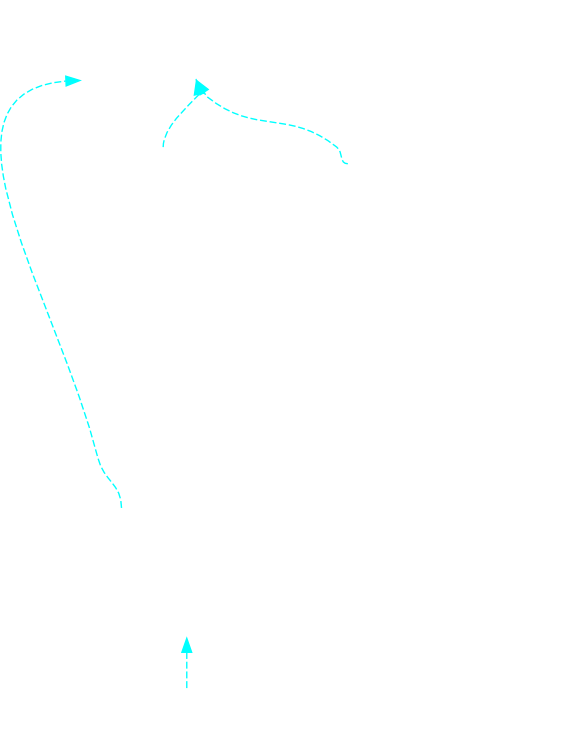
\includegraphics[width = 0.8\textwidth]{examples/ex1-entry-selection-dag.png}
    \end{block}
\end{columns}    

\end{frame}

%%%%%%%%%%%%%%%%%%%%%%%%%%%%%%%%%%%%%%%%%%%%%%%%%%%%%%%%%%%%%%%%%%%%%%%%%%%%%%%%

\begin{frame}[fragile]{Calling convention lowering: The big picture}

\begin{columns}[t]
\column{.5\textwidth}
    LowerFormalArguments()
    \begin{itemize}
        \item Lowers incoming arguments into the DAG
    \end{itemize}

    LowerReturn()
    \begin{itemize}
        \item Lowers outgoing return values into the DAG
    \end{itemize}
    
\column{.5\textwidth}
    % FIXME Add 'a', 'b', 'c' circles and arrows from Lower*() to white circles
    \begin{block}{}
        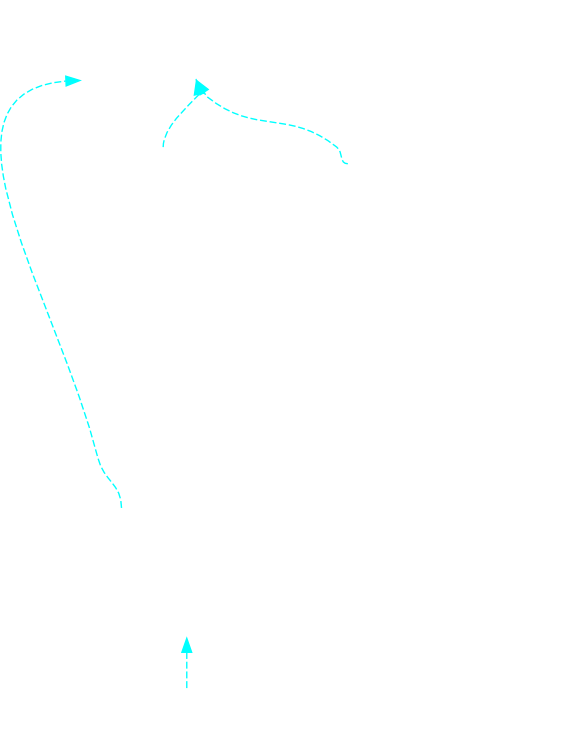
\includegraphics[width = 0.8\textwidth]{examples/ex1-entry-selection-dag.png}
    \end{block}
\end{columns}    

\end{frame}

%%%%%%%%%%%%%%%%%%%%%%%%%%%%%%%%%%%%%%%%%%%%%%%%%%%%%%%%%%%%%%%%%%%%%%%%%%%%%%%%

\begin{frame}[fragile]{Calling convention lowering: LowerFormalArguments()}

\begin{itemize}
    \item Assigns locations to arguments, according to the TableGen-defined calling convention
    \item Creates DAG nodes for each location:
    \begin{itemize}
        \item Registers: CopyFromReg nodes
        \item Stack: frame indices and stack loads
    \end{itemize}
\end{itemize}

\begin{block}{LEGISelLowering.cpp}
\begin{lstlisting}
// LEGTargetLowering::LowerFormalArguments()
SmallVector<CCValAssign, 16> ArgLocs;
CCState CCInfo(CallConv, isVarArg, DAG.getMachineFunction(),
               getTargetMachine(), ArgLocs,
               *DAG.getContext());
CCInfo.AnalyzeFormalArguments(Ins, CC_LEG);
...
\end{lstlisting}
\end{block}

\end{frame}

%%%%%%%%%%%%%%%%%%%%%%%%%%%%%%%%%%%%%%%%%%%%%%%%%%%%%%%%%%%%%%%%%%%%%%%%%%%%%%%%

\begin{frame}{Calling convention lowering: LowerReturn()}

\begin{itemize}
    \item Similar to LowerFormalArguments(), but the other way around
    \item Define another, 'RetCC\_LEG, TableGen calling convention
    \item Call 'AnalyzeReturn()' with it
    \item Walk the return value locations and issue DAG nodes
    \item Return LEGISD::RET instruction
\end{itemize}

\end{frame}

%%%%%%%%%%%%%%%%%%%%%%%%%%%%%%%%%%%%%%%%%%%%%%%%%%%%%%%%%%%%%%%%%%%%%%%%%%%%%%%%

\begin{frame}{Calling convention lowering: LowerCall()}

\begin{itemize}
    \item Hybrid of LowerFormalArguments() and LowerReturn()
    \item Not explicitly covered here
\end{itemize}

\end{frame}

%%%%%%%%%%%%%%%%%%%%%%%%%%%%%%%%%%%%%%%%%%%%%%%%%%%%%%%%%%%%%%%%%%%%%%%%%%%%%%%%

\begin{frame}{Describing instructions: Overview}

\begin{itemize}
    \item Let's start with a simple instruction: ADDrr
    \item Define it in lib/Target/LEG/LEGInstrInfo.td
    \item What we need to specify:
    \begin{itemize}
        \item Operands
        \item Assembly string
        \item Instruction pattern
    \end{itemize}
\end{itemize}

\end{frame}

%%%%%%%%%%%%%%%%%%%%%%%%%%%%%%%%%%%%%%%%%%%%%%%%%%%%%%%%%%%%%%%%%%%%%%%%%%%%%%%%

\begin{frame}[fragile]{Describing instructions: Operands}

\begin{itemize}
    \item List of definitions or outputs ('outs')
    \item List of uses or inputs ('ins')
    \item Operand class:
    \begin{itemize}
        \item Register class (e.g. GRRegs)
        \item Immediate (e.g. i32imm)
        \item More complex operands (e.g. reg + imm for load/store)
    \end{itemize}
\end{itemize}

% FIXME formatting, move to file
\begin{block}{LEGInstrInfo.td}
\begin{lstlisting}
def ADDrr : InstLEG<(outs GRRegs:$dst),
                    (ins GRRegs:$src1, GRRegs:$src2),
                    "add $dst, $src1, $src2",
                    [(set i32:$dst, (add i32:$src1, i32:$src2))]>;
\end{lstlisting}
\end{block}

\end{frame}

%%%%%%%%%%%%%%%%%%%%%%%%%%%%%%%%%%%%%%%%%%%%%%%%%%%%%%%%%%%%%%%%%%%%%%%%%%%%%%%%

\begin{frame}[fragile]{Describing instructions: Selection Patterns}

\begin{itemize}
    \item Matches nodes in the SelectionDAG
    \begin{itemize}
        \item Nodes get turned into MachineInstrs during ISel
        \item If pattern is omitted, selection needs to be done in C++
    \end{itemize}
    \item Syntax:
    \begin{itemize}
        \item One pair of parenthesis defines one node
        \item Nodes have DAG operands, with 'MVT' type (e.g. i32)
        \item Map DAG operands to MI operands
    \end{itemize}
\end{itemize}

% FIXME formatting, move to file
\begin{block}{LEGInstrInfo.td}
\begin{lstlisting}
def ADDrr : InstLEG<(outs GRRegs:$dst),
                    (ins GRRegs:$src1, GRRegs:$src2),
                    "add $dst, $src1, $src2",
                    [(set i32:$dst, (add i32:$src1, i32:$src2))]>;
\end{lstlisting}
\end{block}

\end{frame}

%%%%%%%%%%%%%%%%%%%%%%%%%%%%%%%%%%%%%%%%%%%%%%%%%%%%%%%%%%%%%%%%%%%%%%%%%%%%%%%%

\begin{frame}[fragile]{Describing instructions: Result}

\begin{itemize}
    \item This is what we get after defining the pattern:
    \item Assembly was generated by the instruction printer
    \begin{itemize}
        \item More on this later
    \end{itemize}
\end{itemize}

% FIXME move to file
\begin{block}{ex1.s}
\begin{lstlisting}
# BB#0:                                 # %entry
	add r0, r0, r1
\end{lstlisting}
\end{block}

% FIXME formatting, move to file
\begin{block}{LEGInstrInfo.td}
\begin{lstlisting}
def ADDrr : InstLEG<(outs GRRegs:$dst),
                    (ins GRRegs:$src1, GRRegs:$src2),
                    "add $dst, $src1, $src2",
                    [(set i32:$dst, (add i32:$src1, i32:$src2))]>;
\end{lstlisting}
\end{block}

\end{frame}

%%%%%%%%%%%%%%%%%%%%%%%%%%%%%%%%%%%%%%%%%%%%%%%%%%%%%%%%%%%%%%%%%%%%%%%%%%%%%%%%

\begin{frame}[fragile]{Constants}

\begin{itemize}
    \item Compiling this IR produces the following error:
\end{itemize}

\begin{block}{ex2.ll}
\begin{lstlisting}
%2 = add nsw i32 %1, 2
\end{lstlisting}
\end{block}

\begin{block}{}
\begin{lstlisting}
LLVM ERROR: Cannot select: 0x29d4350: i32 = Constant<2> [ID=2]
In function: main
\end{lstlisting}
\end{block}

\begin{itemize}
    \item Specify how to generate ('materialize') constants
    \item For example, with a 'move' instruction
    \begin{itemize}
        \item E.g. MOVW on ARM for 16-bit constants
    \end{itemize}
\end{itemize}

\end{frame}

%%%%%%%%%%%%%%%%%%%%%%%%%%%%%%%%%%%%%%%%%%%%%%%%%%%%%%%%%%%%%%%%%%%%%%%%%%%%%%%%

\begin{frame}[fragile]{Constants}

\begin{itemize}
    \item Let's define this move instruction:
\end{itemize}

\begin{block}{LEGInstrInfo.td}
\begin{lstlisting}
def MOVWi16 : InstLEG<(outs GRRegs:$dst),
                      (ins i32imm:$src),
                      "movw $dst, $src",
                      [(set i32:$dst, i32imm:$src)]> {
  let isMoveImm = 1;
}
\end{lstlisting}
\end{block}

\begin{itemize}
    \item The previous example translates to:
\end{itemize}

\begin{block}{ex2-ADDrr-MOVW.s}
\lstinputlisting[firstline=7,lastline=8]{examples/ex2-ADDrr-MOVW.s}
\end{block}

\end{frame}

%%%%%%%%%%%%%%%%%%%%%%%%%%%%%%%%%%%%%%%%%%%%%%%%%%%%%%%%%%%%%%%%%%%%%%%%%%%%%%%%

\begin{frame}[fragile]{Constants}

\begin{itemize}
    \item What if instructions take immediates?
\end{itemize}

% FIXME color formatting
\begin{block}{LEGInstrInfo.td}
\begin{lstlisting}
def LEGimm8 : Operand<i32>, ImmLeaf<i32, [{
  return Imm >= 0 && Imm < 256;
}]>;

def ADDri : InstLEG<(outs GRRegs:$dst),
                    (ins GRRegs:$src1, i32imm:$src2),
                    "add $dst, $src1, $src2",
                    [(set i32:$dst, (add i32:$src1, 
                                     LEGimm8:$src2))]>;
\end{lstlisting}
\end{block}

\begin{block}{ex2-ADDri.s}
\lstinputlisting[firstline=7,lastline=7]{examples/ex2-ADDri.s}
\end{block}

\end{frame}

%%%%%%%%%%%%%%%%%%%%%%%%%%%%%%%%%%%%%%%%%%%%%%%%%%%%%%%%%%%%%%%%%%%%%%%%%%%%%%%%

\begin{frame}[fragile]{Matching multiple DAG nodes}

\begin{itemize}
    \item DAG nodes can be nested inside selection patterns
    \begin{itemize}
        \item The output of one node is the input of another
    \end{itemize}
    \item Allows operations to be combined
    \begin{itemize}
        \item Reduces the number of generated instructions
        \item Possibly improves performance or power consumption
    \end{itemize}
    \item Example: multiply and add instruction (ex3.ll)
\end{itemize}

% FIXME color formatting
\begin{block}{LEGInstrInfo.td}
\begin{lstlisting}
def MLA : InstLEG<(outs GRRegs:$dst),
                  (ins GRRegs:$src1, GRRegs:$src2, GRRegs:$src3),
                  "mla $dst, $src1, $src2, $src3",
                  [(set i32:$dst,
                   (add (mul i32:$src1, i32:$src2), i32:$src3))]>;
\end{lstlisting}
\end{block}

\end{frame}

%%%%%%%%%%%%%%%%%%%%%%%%%%%%%%%%%%%%%%%%%%%%%%%%%%%%%%%%%%%%%%%%%%%%%%%%%%%%%%%%

\begin{frame}[fragile]{Matching multiple DAG nodes}

% FIXME center image, add dotted line circles, arrows
% FIXME also add text "With MLA pattern" and assembly output, "Without" etc
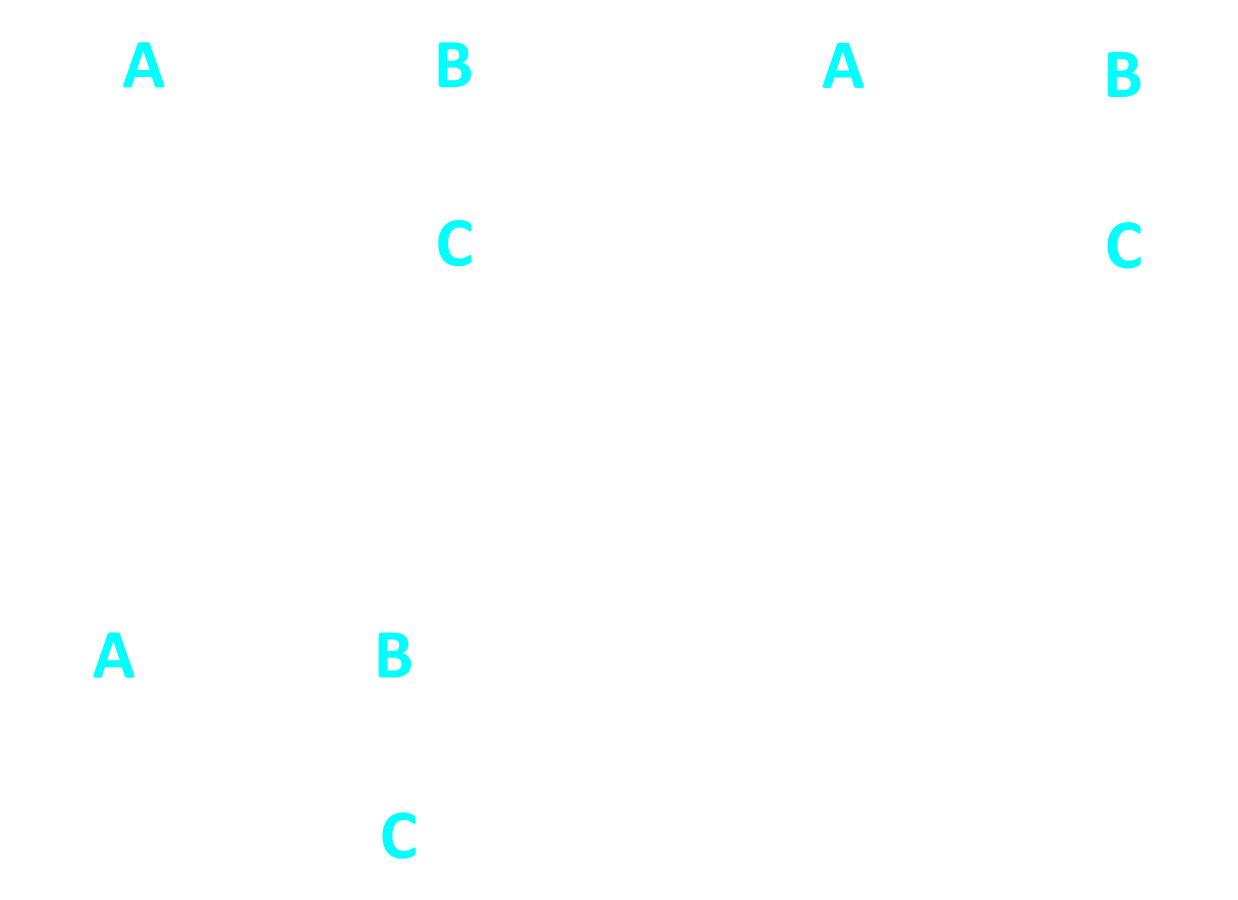
\includegraphics[width = 0.80\textwidth]{examples/ex3-selection1.png}

\end{frame}

%%%%%%%%%%%%%%%%%%%%%%%%%%%%%%%%%%%%%%%%%%%%%%%%%%%%%%%%%%%%%%%%%%%%%%%%%%%%%%%%

\begin{frame}{Frame lowering}

\begin{itemize}
    \item Hooks invoked when values are stored on the stack
    \begin{itemize}
        \item In debug builds (-O0), but not only
    \end{itemize}
    \item Adjust the stack at the beginning ('prologue') and end ('epilogue') of functions
    \begin{itemize}
        \item LEGFrameLowering::emitPrologue()
        \item LEGFrameLowering::emitEpilogue()
    \end{itemize}
    \item Usually by increasing or decreasing the stack pointer
    \item May need to align the stack pointer too
\end{itemize}

\end{frame}

%%%%%%%%%%%%%%%%%%%%%%%%%%%%%%%%%%%%%%%%%%%%%%%%%%%%%%%%%%%%%%%%%%%%%%%%%%%%%%%%

\begin{frame}{Frame lowering}

\begin{itemize}
    \item Example that uses the stack:
\end{itemize}

\begin{block}{ex4.ll}
\lstinputlisting[firstline=7,lastline=10]{examples/ex4.ll}
\end{block}

\begin{itemize}
    \item Output when compiled with -O2:
\end{itemize}

\begin{block}{ex4-O2.s}
\lstinputlisting[firstline=7,lastline=11]{examples/ex4-O2.s}
\end{block}

\end{frame}

%%%%%%%%%%%%%%%%%%%%%%%%%%%%%%%%%%%%%%%%%%%%%%%%%%%%%%%%%%%%%%%%%%%%%%%%%%%%%%%%

\begin{frame}[fragile]{Frame lowering}

\begin{itemize}
    \item When compiling with  -O0, hooks need to be defined
    \item Emit load/store instructions with frame indices
    \item Minimal implementation:
\end{itemize}

\begin{block}{LEGFrameLowering.cpp}
\begin{lstlisting}
// LEGInstrInfo::storeRegToStackSlot()
BuildMI(MBB, I, I->getDebugLoc(), get(LEG::STR))
  .addReg(SrcReg, getKillRegState(KillSrc))
  .addFrameIndex(FrameIndex).addImm(0);

// LEGInstrInfo::loadRegFromStackSlot()
BuildMI(MBB, I, I->getDebugLoc(), get(LEG::LDR), DestReg)
  .addFrameIndex(FrameIndex).addImm(0);

// LEGInstrInfo::copyPhysReg()
BuildMI(MBB, I, I->getDebugLoc(), get(LEG::MOVrr), DestReg)
  .addReg(SrcReg, getKillRegState(KillSrc));
\end{lstlisting}
\end{block}

\end{frame}
